%%%%%%%%%%%%%%%%%%%%%%%%%%%%%%%%%%%%%%%%%%%%%%%%%%%%%%%%%%%%%%
%%% Set Up file
%%%%%%%%%%%%%%%%%%%%%%%%%%%%%%%%%%%%%%%%%%%%%%%%%%%%%%%%%%%%%%

\documentclass[a4paper,12pt]{report}
\textheight=23.5cm
\textwidth=15cm

%\addtolength{\voffset}{-50pt} %edit individual page dimensions
\addtolength{\topmargin}{-.75in}
\addtolength{\textheight}{.3in}

%\clubpenalty=10000
%\widowpenalty=10000
\hyphenpenalty=10000 %Prevent hyphenation if word is too long for line
\tolerance=2000 %How much white space is considered acceptable
\emergencystretch=10pt %Allow 10pt of additional white space per line in order to avoid underfull/overfull lines

\raggedbottom
\pdfminorversion=6

% Text formatting %%%%%%%%%%%%%%%%%%%%%%%%%%%%%%%%%%%%%%%%%%%%%

% Headers and footers
\usepackage{fancyhdr}
\pagestyle{fancy} %Change the style of the current page
\setlength{\headheight}{28pt}
\fancyhead{}
\renewcommand{\chaptermark}[1]{\markboth{#1}{}} %Print the name of the chapter
%\renewcommand{\sectionmark}[1]{\markright{\thesection\ #1}} %Print the name of the section
\fancyhead[L]{\color{Gray}\bfseries\scshape\leftmark} %Current chapter printed on top left
%\fancyhead[R]{\color{Gray}\itshape\rightmark} %Current chapter printed on top left

\renewcommand{\footrulewidth}{0.4pt}
\fancyfoot{}
\fancyfoot[R]{\bfseries\thepage} %Page number on bottom right
\fancypagestyle{plain}{
		\fancyhead{}
		\fancyfoot[R]{\bfseries\thepage}
		\renewcommand{\headrulewidth}{0pt}}

%SI units
\usepackage{siunitx}

% Line settings
\usepackage{setspace}
\usepackage{parskip}
\usepackage{enumitem}

% Colour text
\usepackage[usenames, dvipsnames]{color} %Add colour to text
\usepackage[usenames,dvipsnames,table]{xcolor}

% Chapter headings
\usepackage{titlesec}
\titlespacing*{\chapter}{0cm}{-1.cm}{-40pt}% left margin before-sep after-sep
\titleformat{\chapter}[display] % paragraph shape
	{\color{Gray}\Huge\filleft\scshape} % format for title, label, and text
	{ \normalfont\bf\fontfamily{put}\fontseries{b}\fontsize{95pt}	{0pt} \selectfont\thechapter} % specify label
	{5pt} % separation between label and title body
	{} % before-code
	[\titlerule\vspace{2ex}\filright\vspace{2ex}] % after-code

% Other
\usepackage{kpfonts}
\usepackage{gensymb} %Allows you to use \degree

%Bibliography
\AtBeginDocument{\renewcommand{\bibname}{References}}

%%% Graphics & Figures %%%%%%%%%%%%%%%%%%%%%%%%%%%%%%%%%
\usepackage{float} % Places float at precisely the location in the LaTex code
\usepackage[font=small, labelfont=bf]{caption} %Small captions in bold

% Figures
\usepackage{graphicx}
\usepackage{caption} %Subfigures over a page
\usepackage[position=b]{subcaption}
\usepackage{rotating} %Allows you to rotate floats
\usepackage{rotfloat} %Allows [H] to be used when rotating floats

% Numbering of appendix figures
\usepackage{chngcntr}

% Tables %%%%%%%%%%%%%%%%%%%%%%%%%%%%%%%%%%%%%%%%%%%%
\usepackage{lscape} %landscape tables
\usepackage{tabulary} %Allows you to wrap text in a table column
\tymin=.1\textwidth
\tymax=.7\textwidth
\usepackage{array} %Needed for some functions in tabular
\usepackage{fixltx2e} %Allows you to use \textsubscript in tables
\usepackage{longtable} %Tables can span across multiple pages
\usepackage{booktabs} %Allows you to use \toprule etc when converting excel tables to latex
\usepackage{tabu}
\usepackage{setspace} %Set spacing in longtable
\usepackage{multirow} %Multirows in tables

% Table of contents %%%%%%%%%%%%%%%%%%%%%%%%%%%%%%%%%%%%%%%
% Mini table of contents for each chapter
\usepackage{titletoc}

%References %%%%%%%%%%%%%%%%%%%%%%%%%%%%%%%%%%%%%%%%%
\usepackage{url} %Allows you to add urls
\usepackage{nameref} %Allows you to name chapter in reference rather than number
\usepackage[colorlinks=false, hidelinks]{hyperref} %Citations are turned into hypertext links
\usepackage[backend=bibtex, style=authoryear, maxcitenames=2, mincitenames=1, minbibnames=3, maxbibnames=3, dashed=false, firstinits=true, doi=false, url=false, isbn=false, uniquename=init]{biblatex}
\addbibresource{./ThesisBibliography} %Location of references
\renewbibmacro{in:}{} %Suppress the use of "`in"' before the journal title in bibliography
\DeclareNameAlias{sortname}{last-first} %Display all authors in bibliography as last name followed by first
\renewcommand*{\bibpagespunct}{\addcolon\space} %colon instead of comma before pages in bibliography
\AtEveryBibitem{\clearfield{number}} %remove number field from bibliography

\setcounter{tocdepth}{1}

\begin{document}

\begin{titlepage}
\vspace*{10mm}
	\begin{center}
		\rule[0.5ex]{\linewidth}{2pt}\vspace*{-\baselineskip}\vspace*{3.2pt}
		\rule[0.5ex]{\linewidth}{1pt}\\[\baselineskip]

{\LARGE{\textbf{An integrated metagenomic approach to investigating disease heterogeneity in sepsis due to community acquired pneumonia}}}\\[4mm]

\rule[0.5ex]{\linewidth}{1pt}\vspace*{-\baselineskip}\vspace{3.2pt}
\rule[0.5ex]{\linewidth}{2pt}\\
\vspace{20mm}

{\Large Cyndi Goh}\\

\vspace{6mm}

\includegraphics[scale=0.3]{./oxford_logo-eps-converted-to.pdf}\\
\vspace{6mm}

{\Large Linacre College}\\
\vspace{4mm}
{\large\textsc{University of Oxford}}\\
\vspace{10mm}

\begin{minipage}{10cm}
\begin{center}
{\large A thesis submitted in partial fulfilment of the requirements for the degree of Doctor of Philosophy}
\end{center}
\end{minipage}\\

\vspace{9mm}
{\large\textsc{Michaelmas Term, 2019}}
\vspace{12mm}

\end{center}
\end{titlepage}

\newpage

\chapter*{Abstract} %Creates chapter title but doesn't number
\addcontentsline{toc}{chapter}{\numberline{}Abstract} %Add abstract to table of contents
\thispagestyle{plain}
\pagenumbering{roman} \setcounter{page}{1}
\onehalfspacing
\vspace*{0.4cm}
\begin{center}
{\large\bf An integrated metagenomic approach to investigating disease heterogeneity in sepsis due to community acquired pneumonia} \\
{Cyndi Goh, Linacre College, Michaelmas Term, 2019}\\
\vspace*{0.4cm}
{\itshape A thesis submitted in partial fulfilment of the requirements
for the degree of Doctor of Philosophy of the University of Oxford} \\
\vspace*{0.4cm}
\end{center}

\singlespacing

Sepsis is defined as life-threatening organ dysfunction caused by a dysregulated host response to infection. It is an increasing global burden associated with high mortality, long-term disability and shortened life expectancy. Clinical management of sepsis remains supportive rather than curative and progress in sepsis research has been severely constrained by a heterogeneous disease phenotype, limiting the interpretation of clinical trials and the development of effective therapeutic interventions. One source of heterogeneity is the pathogen but the frequent failure of clinical microbiology to identify the infecting organism in sepsis has limited efforts to understand the effect of disease heterogeneity involving the pathogen. Community-acquired pneumonia (CAP) is the most common cause of sepsis and clinical microbiology is unable to provide a diagnosis in approximately 60\% of cases, suggesting that alternative methods such as clinical metagenomics are required for improved diagnostics. 

Clinical metagenomics involves the application of next-generation sequencing technologies to characterise all the DNA and/or RNA present in a sample, enabling analysis of the entire microbiome as well as the human host genome or transcriptome from patient samples. This thesis presents the development and validation of \textit{Castanet}, a method for targeted metagenomic sequencing using probe-based enrichment. Clinical metagenomic data is presented for 573 patients admitted to intensive care with sepsis due to CAP, including 447 patients for whom clinical microbiology did not identify a pathogen. In addition, droplet digital PCR data is presented for the most frequently identified bacteria (\textit{Streptococcus pneumoniae}) and virus (Epstein-Barr virus) in the metagenomic cohort. Finally, this thesis explores how improved resolution of microbiology in the sepsis cohort can be applied to transcriptomic and genomic-based approaches to understand the host response in sepsis. This includes exploration of Epstein-Barr virus reactivation, differential gene expression analysis for different pathogens, and analysis of the association between specific HLA alleles and susceptibility to different pathogens.

This thesis demonstrates the usefulness of integrating metagenomic data with other omic approaches to enable improved understanding of the heterogeneous host response in sepsis, with opportunities for a precision medicine approach.


 







\newpage
\chapter*{Acknowledgements}
\addcontentsline{toc}{chapter}{\numberline{}Acknowledgements}
\thispagestyle{plain}
\noindent
\singlespacing

Firstly, I would like to thank my two supervisors Julian Knight and Ellie Barnes. Julian has made the Knight group a very happy place to spend four years of my life and I am grateful to him for his patience and guidance, and always having time for me despite the busyness of running a large group. During a period of illness, I particularly appreciated Ellie's wisdom and support.

Members of the Knight group have also provided me with immense support. Special thanks must go to Katie Burnham who has been endlessly willing to share scripts, troubleshoot problems big and small and point me in the right direction. 

I have also been enormously grateful for the care and support I received from Dr Rose Freeman, Dr Evie Kemp, Dr Desi Choi, and Dr Rebecca Knowles Bevis. This DPhil would not have been possible without you. 

Finally, thanks must go to my cycling buddies Becca Kearney and Mimi Harrison who have helped me maintain my sanity on two-wheeled trips involving cake. My family, Mum, Wendi and Jeremy have been an endless source of love and support. And of course, Oscar who never fails to cheer me up with licks and cuddles.







\newpage
\chapter*{Declarations}
\addcontentsline{toc}{chapter}{\numberline{}Declarations}
\thispagestyle{plain}
\noindent

I declare that, unless otherwise stated, all work presented in this thesis is my own. Several aspects of the study relied upon collaboration where part of the work was conducted with or by others.

\textbf{Study recruitment}: The Genomic Advances in Sepsis (GAinS) study began recruiting patients in 2005 from 34 intensive care units across the UK. From October 2015, I have been responsible for liaising with research nurses, providing supplies, maintaining sample records, and collecting and processing samples.

\textbf{Pathogen probes}: Probe design was carried out by Azim Ansari. Curation of meningitis pathogen sequences from RefSeq was performed by Ivo Elliott. Curation of additional pneumonia pathogen sequences was performed by myself. 

\textbf{Metagenomics}: I carried out the nucleic acid extractions (supervised by Anthony Brown) and library preparation (supervised by Amy Trebes) for the initial two optimisation experiments and 32 metagenomic samples. Nucleic acid extractions for the subsequent samples were carried out by Anthony Brown and George Macintyre. Library preparation for the remainining samples were carried out by Hubert Slawinski and Mariateresa de Cesare. Data processing and analysis was performed in collaboration with Tanya Golubchik.

\textbf{Cardiac surgery patients}: The cardiac surgery patients were recruited by Eduardo Svoren and Bart's and the London NHS Trust.

\textbf{Axiom microbiome array}: Library preparation was performed by Hannah Matten.

\textbf{Gene expression}: RNA sample processing was performed by Yuxin Mi, Alice Allcock, Katie Burnham, Emma Davenport, Jayachandran Radhakrishnan, Narelle Magueri, and Ashley Thorpe. Microarray gene expression data was generated by the Wellcome Sanger Institute (WSI) and Wellcome Centre for Human Genetics (WHG) Core Genomics facilities.

\textbf{HLA work}: probe design was carried out by Azim Ansari. Library preparation for HLA enrichment experiments were performed by Mariateresa de Cesare. DNA samples were processed by myself, Yuxin Mi, Andrew Kwok, Alice Allcock, Katie Burnham, Jayachandran Radhakrishnan, Emma Davenport, Anna Rautanen, and Tara Mills. Genotyping data was generated by the WHG and WSI Core Genomics facilities. Genotyping QC was performed by Emma Davenport and Katie Burnham. SNP2HLA imputation was performed by Justin Whalley.

\newpage

\chapter*{Submitted Abstracts}
\addcontentsline{toc}{chapter}{\numberline{}Submitted Abstracts}
\thispagestyle{plain} %Removes the header

\noindent
\textbf{Quest for the one true test: enrichment-based metagenomic sequencing in paediatric meningitis and adult sepsis}\\
Oral: Applied Bioinformatics and Public Health Microbiology (2019)\\
T Golubchik, \textbf{C Goh}, MA Ansari, M de Cesare, A Trebes, D Bonsall, A Brown, M Sadarangani, P Piazza, K Jolley, I Elliott, C Ip, H Slawinski, A Coxon, G Meddaugh, P Hutton, CJ Hinds, E Barnes, AJ Pollard, JC Knight, R Bowden\\

\textbf{Using \textit{in vivo} eQTL interactions to identify the regulatory drivers of variation in the transcriptomic response to sepsis}\\
Poster: Immunogenomics of Disease: Accelerating to Patient Benefit (2019)\\
EE Davenport, KL Burnham, \textbf{C Goh}, J Radhakrishnan, P Hutton, TC Mills, A Rautanen, AC Gordon, N Soranzo, AVS Hill, CJ Hinds, S Raychaudhuri, JC Knight\\

\textbf{Using \textit{in vivo} eQTL interactions to identify the genetic drivers of the transcriptomic response to sepsis}\\
Poster: American Society of Human Genetics (2018)\\
EE Davenport, KL Burnham, \textbf{C Goh}, J Radhakrishnan, P Hutton, TC Mills, A Rautanen, AC Gordon, N Soranzo, AVS Hill, CJ Hinds, S Raychaudhuri, JC Knight\\

\newpage
\chapter*{Associated Publications}
\addcontentsline{toc}{chapter}{\numberline{}Associated Publications}
\thispagestyle{plain}

\noindent
\textbf{Enhanced understanding of the host-pathogen interaction in sepsis: new opportunities for omic approaches}\\
The Lancet Respiratory Medicine 2017; 5: 212-23\\
\textbf{C Goh}, JC Knight\\

\textbf{Targeted metagenomic sequencing enhances the identification of pathogens associated with acute infection}\\
Nature Microbiology (under review), bioRxiv (2019) /textit{https://doi.org/10.1101/716902}\\
\textbf{C Goh}, T Golubchik, MA Ansari, M de Cesare, A Trebes, I Elliott, D Bonsall, P Piazza, A Brown, H Slawinski, N Martin, S Defres, MJ Griffiths, JE Bray, MC Maiden, P Hutton, CJ Hinds, T Solomon, E Barnes, AJ Pollard, M Sadarangani, JC Knight, R Bowden\\

\textbf{Epstein-Barr virus reactivation in sepsis is associated with an immunosuppressed host transcriptomic endotype}\\
Critical Care (under review)\\
\textbf{C Goh}, KL Burnham, MA Ansari, M de Cesare, T Golubchik, P Hutton, LE Overend, EE Davenport, CJ Hinds, R Bowden, JC Knight\\


\newpage
\addcontentsline{toc}{chapter}{\numberline{}Contents}
\tableofcontents

\newpage
\listoffigures
\addcontentsline{toc}{chapter}{\numberline{}List of Figures}

\newpage
\listoftables
\addcontentsline{toc}{chapter}{\numberline{}List of Tables}

\chapter*{Abbreviations}
\addcontentsline{toc}{chapter}{\numberline{}Abbreviations}

\begin{longtable}[l]{l l}

		\textbf{APACHE-II} & Acute physiology and chronic health evaluation II\\
		\textbf{AST} & Antimicrobial stewardship team\\
		\textbf{AUC} & Area under the curve\\
		\textbf{bp} & Base pairs\\
		\textbf{BWA} & Burrows-Wheeler Aligner\\
		\textbf{CAP} & Community-acquired pneumonia\\
		\textbf{cDNA} & Complementary deoxyribonucleic acid\\
		\textbf{CF} & Combined with fragmentation\\
		\textbf{ChiMES} & Childhood meningitis and encephalitis study\\
		\textbf{CI} & Confidence interval\\
		\textbf{CLiMax} & Confidence likelihood maximisation\\
		\textbf{CMV} & Cytomegalovirus\\
		\textbf{CnoF} & Combined with no fragmentation\\
		\textbf{CSF} & Cerebrospinal fluid\\
		\textbf{ddPCR} & Digital droplet PCR\\
		\textbf{DNA} & Deoxyribonucleic acid\\
		\textbf{DNase} & Deoxyribonuclease\\
		\textbf{dsDNA} & Double-stranded deoxyribonucleic acid\\
		\textbf{dsRNA} & Double-stranded ribonucleic acid\\
		\textbf{EBV} & Epstein-Barr virus\\
		\textbf{eCRF} & Electronic case record form\\
		\textbf{EDTA} & Ethylenediaminetetraacetic acid\\
		\textbf{ELISA} & Enzyme-linked immunosorbent assay\\
		\textbf{EPIC} & Aetiology of pneumonia in the community\\
		\textbf{eQTL} & Expression quantitative trait loci\\
		\textbf{ERCC} & External ribonucleic acid controls consortium\\
		\textbf{ESI-MS} & Electrospray ionisation mass spectrometry\\
		\textbf{FDR} & False discovery rate\\
		\textit{\textbf{FER}} & Fes/Fps related tyrosine kinase\\
		\textbf{GAinS} & Genomic advances in sepsis\\
		\textbf{GWAS} & Genome-wide association study\\
		\textbf{GWLS} & Genome-wide linkage study\\
		\textbf{HBV} & Hepatitis B virus\\
		\textbf{HCV} & Hepatitis C virus\\
		\textbf{HHV6} & Human herpesvirus 6\\
		\textbf{HIV} & Human immunodeficiency virus\\
		\textbf{HLA} & Human leukocyte antigen\\
		\textbf{HR} & Hazard ratio\\
		\textbf{HSV} & Herpes simplexvirus\\
		\textbf{HWE} & Hardy-Weinberg equilibrium\\
		\textbf{ICU} & Intensive care unit\\
		\textbf{IPA} & Ingenuity pathway analysis\\
		\textbf{IRF} & Interferon regulatory factor\\
		\textbf{MAF} & Minor allele frequency\\
		\textbf{MAFFT} & Multiple alignment using fast Fourier transform\\
		\textbf{MALDI-TOF} & Matrix-associated laser desorption/ionisation-time of flight\\
		\textbf{MARS} & Molecular diagnosis and risk stratification of sepsis\\
		\textbf{MHC} & Major histocompatibility complex\\
		\textbf{MiDAS} & Microbial detection analysis software\\
		\textbf{miRNA} & Micro ribonucleic acid\\
		\textbf{MOSAIC} & Mechanisms of Severe Acute Influenza Consortium\\
		\textbf{MR} & Misclassification rate\\
		\textbf{NCBI} & National centre for biotechnology information\\
		\textbf{NGS} & Next-generation sequencing\\
		\textbf{NIBSC} & National institute for biological standards and control\\
		\textbf{NS1} & Non-structural protein 1\\
		\textbf{nt} & Nucleotide\\
		\textbf{PBWT} & Positional Burrows-Wheeler Transform\\
		\textbf{PC} & Principal component\\
		\textbf{PCA} & Principal component analysis\\
		\textbf{PCR} & Polymerase chain reaction\\
		\textbf{pHBV} & Hepatitis B virus plasmid\\
		\textbf{pQTL} & Protein quantitative trait loci\\
		\textbf{PRR} & Pattern recognition receptor\\
		\textbf{REALISM} & Reanimation low immune status markers\\
		\textbf{RF} & Random forest\\
		\textbf{rMLST} & Ribosomal multilocus sequence typing\\
		\textbf{RNA} & Ribonucleic acid\\
		\textbf{ROC} & Receiver operating curve\\
		\textbf{rps} & Ribosomal protein subunit\\
		\textbf{rRNA} & Ribosomal ribonucleic acid\\
		\textbf{RSV} & Respiratory syncytial virus\\
		\textbf{SIRS} & Systemic inflammatory response syndrome\\
		\textbf{SNP} & Single nucleotide polymorphism\\
		\textbf{SOFA} & Sequential organ failure assessment\\
		\textbf{SRS} & Sepsis response signature\\
		\textbf{ssRNA} & Single stranded RNA\\
		\textbf{STOP-HCV} & Stratified medicine to optimise the treatment of patients with hepatitis C\\& virus infection\\
		\textbf{SURPI} & Sequence-based ultra-rapid pathogen identification\\
		\textbf{T1DGC} & Type 1 diabetes genetics consortium\\
		\textbf{TTV} & Torque teno virus\\
		\textbf{UK} & United Kingdom\\
		\textbf{USA} & United States of America\\
		\textbf{VANISH} & Vasopressin vs norepinephrine as initial therapy in septic shock\\
		\textbf{VCA} & Viral capsid antigen\\
		\textbf{VMR} & Viral multiplex reference\\
		\textit{\textbf{VPS13A}} & Vacuolar protein sorting 13 homolog A\\
		\textbf{vsn} & Variance stabilisation and normalisation\\
		\textbf{VZV} & Varicella zoster virus\\
		\textbf{WHG} & Wellcome Centre for Human Genetics\\
		\textbf{WSI} & Wellcome Sanger Institute\\
		
		
		

\end{longtable}

\pagenumbering{arabic} 
\setcounter{page}{1}
\doublespacing

%List the subfolders and .tex files for each of the chapters to be included
\chapter{Introduction}
\label{ch:Introduction}
\textit{This chapter presents the aims of this thesis, and provides an overview of pre-existing knowledge relevant to these goals}

% 8595 text, 150 headers

\startcontents[chapters]{\vspace{-1.4cm}}
\singlespacing
\printcontents[chapters]{}{1}{\section*{ }\setcounter{tocdepth}{1}}
\doublespacing
\vspace{0.5cm}

The overall objective of this thesis is to 

\section{Genetics and gene expression}

The human genome was first sequenced completely by the Human Genome Project Consortium in 2003 \parencite{Collins2003}. 

\subsubsection{Types of genetic variation}

A polymorphism is a genetic locus that exists in multiple forms, or alleles, at appreciable frequencies in a population (e.g. minor allele $\geq1\%$). 

\section{Specific aims and objectives}

The aims of this thesis are to:

\begin{itemize}[leftmargin=*]

\item	\textbf{Investigate the host transcriptome in sepsis of different sources 
(\hyperref[ch:Results1]{Ch. 3})} \\
	The two most common causes of sepsis in the UK are community acquired pneumonia (CAP) and faecal peritonitis (FP). The host transcriptome in sepsis due to FP has not yet been described, and the clinical differences observed between CAP and FP suggest that variation may also be observed in the molecular response to disease. I aim to:

		\begin{enumerate}
			\item describe the host transcriptome in sepsis due to FP and CAP for peripheral blood leukocytes
			\item directly compare gene expression between CAP and FP patients
			\item identify temporal changes in gene expression in CAP and FP
		\end{enumerate}

	\item  \textbf{Compare the sepsis transcriptomic response to related conditions 
	(\hyperref[ch:Results1]{Ch. 3})} \\
The sepsis response is related to the systemic inflammatory response to insults such as surgery and trauma. Comparison of the infectious and sterile responses might be aid interpretation of the biological processes involved. I will therefore:
		\begin{enumerate}
				\item define the transcriptomic response in:
					\begin{enumerate}
							\item sepsis due to CAP and FP, in contrast to non-septic samples
							\item traumatic injury, in contrast to healthy volunteers
							\item cardiac surgery, using pre- and post-operative samples
						\end{enumerate}
					\item compare these responses across conditions
				\end{enumerate}
		
\end{itemize} 
										
\cite{Bonsall2015}
\chapter{Materials and Methods}
\label{ch:MandM}
\textit{This chapter describes the patient cohorts, laboratory methods, and bioinformatic methods used in this thesis}

\startcontents[chapters]{\vspace{-1.4cm}}
\singlespacing
\printcontents[chapters]{}{1}{\section*{ }\setcounter{tocdepth}{1}}
\doublespacing

\section{Genomic Advances in Sepsis}
The UK Genomic Advances in Sepsis (GAinS) study (http://ukccggains.com) is a multicentre prospective study initiated in 2005 by the UK Critical Care Genomics group with the original aim of characterising genetic variants that affect susceptibility to and outcomes from sepsis. A bioresource arising from this study includes biological samples and phenotypic information from over 2,000 individuals with sepsis from community acquired pneumonia (CAP) or faecal peritonitis (FP) admitted to intensive care units (ICUs). This thesis focuses only on the subset of individuals with sepsis from CAP. Recruitment was initially carried out in 34 ICUs and remains ongoing in 4 ICUs across the UK.

\subsection{GAinS patient recruitment and exclusion criteria}
Sepsis patients were recruited through the GAinS study from 34 participating ICUs between 2005 and 2019. Patients were recruited if they met the diagnostic criteria for severe sepsis in use at the time of study initiation (Sepsis-2, 2001 American College of Chest Physicians/Society of Critical Care Medicine consensus definition \parencite{Levy2003}).  Sepsis was defined as infection with signs of systemic inflammation \ref{tab:sepsis} and classified as severe when associated with organ dysfunction. CAP was defined as febrile illness associated with cough, sputum production, breathlessness, leukocytosis and radiological features of pneumonia acquired prior to or within 48 hours of hospital admission \parencite{Lim2009}. Exclusion criteria included immunocompromise, admission for palliative care only, and pregnancy.

\begin{landscape}
\begin{table}[htbp]
\begin{center}
\begin{tabular}{ll}
\multicolumn{2}{l}{Infection, documented or suspected, and some of the following:}                                                                                                                                                                                                                                                                                                                                                                                                                                              \\ \hline
General variables           & \begin{tabular}[c]{@{}l@{}}Fever (core temperature \textgreater{}38.3\textdegree C)\\ Hypothermia (core temperature \textless{}36\textdegree C)\\ Heart rate \textgreater{}90/min or \textgreater{}2 SD above the normal value for age\\ Tachypnoea\\ Altered mental status\\ Significant oedema or positive fluid balance (\textgreater{}20 ml/kg for 24 hours)\\ Hyperglycaemia (plasma glucose \textgreater{}7.7 mol/L) in the absence of diabetes\end{tabular}                                                          \\ \hline
Inflammatory variables      & \begin{tabular}[c]{@{}l@{}}Leukocytosis (WBC count \textgreater{}12,000/uL)\\ Leukopenia (WBC count \textless{}4,000/uL)\\ Normal WBC count with \textgreater{}10\% immature forms\\ Plasma C-reactive protein \textgreater{}2 SD above the normal value\\ Plasma procalcitonin \textgreater{}2 SD above the normal value\end{tabular}                                                                                                                                                              \\ \hline
Haemodynamic variables      & \begin{tabular}[c]{@{}l@{}}Arterial hypotension (SBP \textless{}90 mmHg, MAP \textless{}70, or an SBP decrease \textgreater{}40 mm Hg in adults or \textgreater{}2 SD\\below normal for age)\\ SvO$_{2}$ \textgreater{}70\%\\ Cardiac index \textgreater{}3.5 L/min/M$^{2}$\end{tabular}                                                                                                                                                                                                                       \\ \hline
Organ dysfunction variables & \begin{tabular}[c]{@{}l@{}}Arterial hyperaemia (PaO$_{2}$/FiO$_{2}$ \textless{}300 mm Hg)\\ Acute oliguria (urine output \textless 0.5 ml/kg/h or 45 mmol/L for at least 2 hours)\\ Creatinine increase (\textgreater{}0.5 mg/dL)\\ Coagulation abnormalities (INR \textgreater{}1.5 or APTT \textgreater{}60 seconds)\\ Ileus (absent bowel sounds)\\ Thrombocytopenia (platelet count \textless{}100,000/uL)\\ Hyperbilirubinaemia (plasma total bilirubin \textgreater{}4 mg/dL or 70 mmol/L)\end{tabular} \\ \hline
Tissue perfusion variables  & \begin{tabular}[c]{@{}l@{}}Hyperlactataemia (\textgreater{}1 mmol/L)\\ Decreased capillary refill or mottling\end{tabular}                                                                                    
\end{tabular}
\end{center}
\smallskip
\caption[Diagnostic criteria for sepsis]{\textbf{Diagnostic criteria for sepsis.} WBC=white blood cell; SBP=systolic blood pressure; MAP=mean arterial blood pressure; SvO2=mixed venous oxygen saturation; INR=international normalised ratio; APTT=activated partial thromboplastin time}
\label{tab:sepsis}
\end{table}
\end{landscape}

\section{Additional cohorts}
Two other cohorts were studied: (a) patients with hepatitis C virus infection, and (b) patients undergoing cardiac surgery.

\subsection{Hepatitis C virus infection patient recruitment and exclusion criteria}
The hepatitis C virus (HCV) infection cohort was recruited through the NIHR Oxford Biomedical Research Centre Prospective Cohort Study in Hepatitis C virus infection. This aim of this study was phenotypic and genotypic characterisation of a cohort of patients with current and resolved HCV infection. Adult patients were recruited if HCV infection was confirmed by detectable viral RNA or if there was evidence of spontaneously resolved infection confirmed by the presence of HCV antibodies in the absence of detectable HCV RNA. Exclusion criteria included clinician judgment that the patient was unlikely to participate in a long-term study.

\subsection{Cardiac surgery patient recruitment and exclusion criteria}
Patients undergoing elective cardiac surgery requiring cardiopulmonary bypass (coronary artery bypass grafting, valve replacement, or valve repair) were recruited to the Genomic Advances in Cardiac Surgery study by Dr Eduardo Svoren and Professor Charles Hinds (Bart's and the London NHS Trust). This study aimed to investigate the host inflammatory response induced by elective cardiac surgery involving cardiopulmonary bypass. They were included in this thesis as uninfected negative controls for sepsis. Patients were excluded if they were immunocompromised, undergoing an emergency operation, had malignancy, or were unable to provide informed consent. 


\section{Metagenomics}
\subsection{Nucleic acid extraction}

Total nucleic acid extraction was performed using the NucliSENS easyMag platform (Biomerieux). Typically, 500 $\mu$l of extracted plasma was eluted in 25 $\mu$l of buffer. Postextraction quality control was performed using the Agilent 2100 Bioanalyzer platform and/or the Qubit dsDNA High Sensitivity Assay (Thermo Fisher Scientific) in a subset of samples.

\subsection{Library preparation methods}
Four library prepration methods were evaluated.

1. RNA: We used the NEBNext Ultra Directional RNA Library Preparation Kit for Illumina (New England Biolabs) with several modifications to the manufacturer’s guidelines including: fragmentation for 4 minutes at 94$^{\circ}$C, omission of Actinomycin D at first-strand reverse transcription, library amplification for 15 PCR cycles using custom indexed primers and post-PCR clean-up with 0.85x volume Ampure XP (Beckman Coulter).

2: DNA: The Nextera DNA Library Preparation Kit (Illumina) was used according to the manufacturer's guidelines.

3: Combined with fragmentation (CF): This involved the RNA protocol (NEBNext Ultra Directional RNA Library Preparation) (1) followed by the DNA protocol (Nextera DNA Library Preparation)(2).

4. Combined with no fragmentation (CnoF): This involved the RNA protocol (1), with omission of fragmentation, end repair, and adaptor ligation steps, followed by the DNA protocol (2). 

\subsection{Spike-ins}
RNA: We used the Ambion ERCC RNA Spike-In Mix 1 (Thermo Fisher Scientific) consisting of 92 synthetic transcripts between 250-2000 nucleotides in length, at a range of pre-specified concentrations (External RNA Controls Consortium 2005).

DNA: Multiple restriction enzyme digest of three synthetic plasmids was performed according to manufacturer instructions (New England BioLabs) (Table ~\ref{tab:plasmid}). 

\begin{table}[htbp]
\begin{center}
\begin{tabular}{|c|c|c|c|}
\hline
Plasmid & Original size (bp) & Restriction enzymes & Fragment sizes (bp)\\
\hline
pHBV & 6820 & AccI, AlwNI, HindIII, NdeI & 800, 1178, 1652, 3190\\
p1990 & 4808 & AccI, AlwNI, HindIII & 401, 588, 1796, 2023\\
p2022 & 3356 & AccI, AlwNI, NdeI & 379, 1099, 1878\\
\hline
\end{tabular}
\end{center}
\smallskip
\caption[DNA plasmid spike-in controls]{\textbf{DNA spike-in controls.} Plasmids, restriction enzymes, and resulting fragment sizes.}
\label{tab:plasmid}
\end{table}

The three plasmids were pooled in equal mass ratios and spiked-in at 3\% sample DNA concentration by mass.

\subsection{Probe-based enrichment}
In collaboration with a paediatric meningitis study, a custom probe panel covering bacterial and viral pathogens relevant to meningitis and pneumonia was designed using the Agilent SureDesign service. This included probes complementary to three ERCC's (External RNA Controls Consortium; ERCC14, ERCC25, ERCC116) and the pHBV plasmid fragment. The probe set included 52,101 120nt RNA oligonucleotide probes (\num{5.87e6} bp). 

1$\mu$g of each indexed pooled library was enriched using the Agilent SureSelect$^{XT}$ Target Enrichment System for Illumina Paired-End Multiplexed Sequencing Library protocol with one major modification to the recommended protocol. This involved capture on a post-PCR indexed pool with use of oligonucleotide blockers complementary to adapter sequences.

\subsection{Data processing}
De-multiplexed sequence read-pairs were trimmed of adapter sequences using Trimmomatic v0.36 \parencite{Bolger2014}. Fastq files containing the trimmed reads were then classified with the metagenomic classifier Kraken v1 \parencite{Wood2014} using a custom database comprised of human, bacterial, viral and fungal genomes. Unclassified reads as well as reads classified as bacterial or viral were aligned using bwa v0.7.12\parencite{Li2009} to a multi-fasta reference comprised of consensus sequences corresponding to the enrichment probe set, sequencing contaminants (e.g. \textit{Alteromonas} species) and potential clinical sample contaminants including non-pathogenic \textit{Streptococcus} species.


\section{Digital droplet PCR}
Digital droplet PCR (ddPCR) was performed for targets from several microorganisms: (a) \textit{S. pneumoniae}, (b) influenza,  (c) Epstein-Barr virus (EBV), and (d) cytomegalovirus (CMV). The assay was performed on samples following nucleic acid extraction as above. For the RNA-based pathogen (influenza) nucleic acid extraction was followed by first strand cDNA synthesis (SuperScript III First-Strand Synthesis System, Invitrogen). 

Sample processing was performed in triplicate (1.5$\mu$l per replicate) following the recommended workflow (QX200 ddPCR system, Bio-Rad). Custom-designed PrimeTime (IDT) primer/probe sets targeting the \textit{S. pneumoniae} capsular polysaccharide biosynthesis (\textit{cpsA}), influenza A matrix (M), EBV Epstein-Barr nuclear antigen 1 (\textit{EBNA-1}), and CMV envelope glycoprotein B (\textit{UL55}) genes were designed based on published sequence data \parencite{Park2010} \parencite{Shu2011} \parencite{Ryan2004} \parencite{Sedlak2014} (Table \ref{tab:ddPCRprobes}). A total of 20$\mu$l of each reaction mixture was loaded onto a DG8 cartridge (Bio-Rad) with 70$\mu$l of droplet generation oil (Bio-Rad) and placed in the QX100 Droplet Generator (Bio-Rad). Droplets were transferred to a 96-well PCR plate and PCR amplification performed on a C1000 Touch Thermal Cycler (Bio-Rad). Following amplification, the plate was loaded onto the QX100 Droplet Reader (Bio-Rad). Data was analysed with the QuantaSoft analysis software.

\section{Epstein Barr Virus Serology}
Enzyme linked immunosorbent assay (ELISA) was used to test for the presence of IgG and IgM antibodies against the EBV viral capsid antigen (VCA) using proprietary kits (Abcam). The manufacturer's instructions were followed. Plasma samples (10$\mu$l) were diluted to the recommended 1:100 concentration and run in duplicate. Absorbance was measured at 450nm using the CLARIOstar plate reader (BMG Labtech). Samples were considered to be positive if the absorbance value was greater than 10\% over the cut-off control absorbance value. 

\section{Axiom Microbiome Array}
Plasma samples from ten individuals were tested on the Axiom Microbiome Array platform (Affymetrix). For each sample, total nucleic acid was extracted from 500$\mu$l plasma and 21 out of the 25$\mu$l eluted product (equivalent to 420$\mu$l plasma) was processed according to the Axiom 2.0 Assay Protocol. Each array includes 1,277,846 target probes and 60,152 random negative control probes. The target probes represent 135,555 sequences from 12,513 microbial species from five domains: archaea, bacteria, fungi, protozoa and viruses. Sample processing involved parallel processing of samples on a microarray plate with isothermal whole-genome amplification, hybridisation to 35-mer oligonucleotide probes, washing and scanning on the GeneTitan Multi-Channel instrument.  Data analysis was performed using the Axiom Microbial Detection Analysis Software (MiDAS) based on a Composite Likelihood Maximisation Method (CLiMax) algorithm. Probes were considered positive if signal intensity exceeded the 99th percentile of the random control probe intensities and if more than 20\% of target-specific probes were detected.  


\section{Transcriptomics}
\subsection{Sample collection}
Serial samples for RNA were obtained by collecting 5ml blood into Vacuette EDTA tubes (Becton Dickinson). Using a vacutainer system, blood was passed across a LeukoLOCK leukocyte enrichment filter (Ambion), isolating the total blood leukocyte population. The filtered leukocytes were stabilised with RNA\textit{later}. Filters were stored and transported at -80\degree C. GAinS samples were collected on days 1, 3, and/or 5 of ICU admission. Cardiac samples were collected prior to induction of anaesthesia, immediately post-operative and 24 hours post-operative.

\subsection{RNA extraction}
RNA extraction was performed using the Total RNA Isolation Protocol (Ambion). Purified RNA, depleted of globin mRNA, was extracted from the LeukoLOCK filters. Filter contents were lysed and eluted with a guanidine thiocyanate-based solution. Degradation of cellular proteins and DNA was carried out using Proteinase K and DNase I respectively. Magnetic bead technology was used to purify the RNA. Spectrophotometry (Nanodrop 2000; Thermo Scientific) was used to quantify the RNA yield and quality of a small subset was evaluated using on-chip electrophoresis (Bioanalyzer; Agilent).

\subsection{Microarray data processing and analysis}
Genome-wide gene expression data was generated on 1000ng RNA using the Illumina Human-HT-12 v4 Expression BeadChip gene expression platform comprising 47,231 probes. The report for analysis was generated by Illumina's Genomestudio software. The four microarray datasets were generated by Dr Jayachandran Radhakrishnan (Radhakrishnan 2010), Dr Emma Davenport (Davenport 2011) and Dr Katie Burnham (Burnham 2014 and Burnham 2016). The first two datasets were generated at the Wellcome Sanger Institute (WSI, Cambridge) whilst the final two datasets were generated at the Wellcome Centre for Human Genetics (WHG, Oxford).

For each dataset, data backgrounds were subtracted and probes with a detection value of \textless 0.95  in \textgreater 95\% of samples were filtered out. The raw data was transformed and normalised using the Variance Stabilisation and Normalisation (vsn) R package \parencite{Huber2002}. QC checks including Principal Component Analysis (PCA) was carried out in R to identify batch and array effects. The four individual datasets were then combined and probe filtering repeated using the parameters described above, followed by normalisation using vsn. The ComBat function from the R package sva \parencite{Leek2012} was used to directly estimate and remove the known batch effects. 

Differential gene expression was analysed using the R package limma \parencite{Ritchie2015}, which fits a generalised linear model to the expression of each gene and uses an empirical Bayes approach to account for overall variance in the dataset. Genes with an FDR \textless 0.05 and $\geq$1.5 were considered to be differentially expressed. Pathway enrichment analysis was carried out with XGR \parencite{Fang2016} using the xEnricherGenes function and taking all genes tested for differential expression as the background. Predictive gene signatures were derived using the elastic net method \parencite{Zou2005} \parencite{Herberg2016}. This variable selection algorithm combines the lasso and ridge regression methods of shrinkage by minimising the number of variables included (lasso) whilst also making the model less dependent on any single variable (ridge).

\section{Genomics}
\subsection{DNA extraction}
DNA was extracted from buffy coat or whole blood using one of three protocols: (a) Qiagen DNA extraction protocol, (b) Maxwell 16 Blood purification kit (Promega), or (c) QIAamp Blood Midi kit protocol (Qiagen). In the Qiagen protocol, cell lysis is followed by sequential removal of unwanted cell components (e.g. protein and RNA). The Maxwell automated protocol uses paramagnetic particles to purify DNA following cell lysis while the QIAamp kit uses a spin column. DNA yield was determined by spectrophotometry (Nanodrop) or fluoresecence using the Quant-iT PicoGreen kit (Invitrogen). 

\subsection{Genotyping and data processing}
Three genome-wide genotyping datasets were generated. The first dataset had previously been generated at the WHG for 295 CAP patients and 63 cardiac surgery patients and 730,525 SNPs using the Illumina HumanOmniExpress BeadChip \parencite{Davenport2014}. The second dataset was generated for 655 patients at the WSI using the Infinium CoreExome BeadChip (Illumina; 551,839 SNPs) and the Illuminus genotype calling algorithm. The third dataset was generated for 307 patients at the WHG using the Infinium Global Screening Array BeadChip (Illumina; 654,027 SNPs).

PLINK was used for the genotyping QC \parencite{Anderson2010}. Samples were excluded on the basis of discordant sex information, proportion of missing genotypes \textgreater 0.02, heterozygosity rate, identity by descent. SNPs were excluded if they had missing data proportion \textgreater 0.05, minor allele frequency (MAF) \textless 0.01, and Hardy-Weinburg equilibrium (HWE) p \textless 1x10$^{-5}$.

\subsection{Imputation}
Each of the genotyping datasets was imputed independently against the Haplotype Reference Consortium (HRC) release 1.1 panel using the Sanger Imputation Service \parencite{McCarthy2016}. Pre-imputation checks were carried out using the HRC Imputation Tool (Will Rayner, WHG; www.well.ox.ac.uk/~wraymer/tools). Genotypes were phased using Eagle 2 \parencite{Loh2016} and imputed using PBWT \parencite{Durbin2014}. SNPs with an info score \textless 0.9 were removed. 

\subsection{HLA enrichment}
127 libraries previously prepared for metagenomic sequencing using the combined no fragmentation protocol described above were enriched for sequencing using a custom designed set of HLA probes designed by Dr Azim Ansari. The enrichment protocol and sequencing are as described for the metagenomic samples.

\subsection{HLA assignment}
For patients with genotyping data, HLA alleles were imputed using the SNP2HLA package \parencite{Jia2013}. Two-digit and four-digit alleles were imputed for the HLA-A, -C, -B, -DRB1, -DQA1, and -DQB1 gene loci within the MHC region on chromosome 6. SNP2HLApackagev1.0.2, Beagle.3.0.4, linkage2beagle2.0 and Plink1.07 were used following recommended parameters with 10 iterations and a marker window size of 1000. The pre-built Type 1 Diabetes Genetics Consortium (T1DGC) reference panel of 5225 European individuals and 8961 binary markers was downloaded along with the SNP2HLA tool and used as a training set for the HLA imputation. As well as the imputed HLA alleles, imputation posterior probabilities were also determined to inform the accuracy of the imputed alleles.

\section{Statistical analysis}
Statistical analysis was carried out in R. Demographic data were compared between groups by $\chi^2$ test for categorical data, t-test for continuous parametric data, Mann-Whitney U-test for continuous non-parametric data, and log rank test for survival. ROC curves were plotted using the pROC R package \parencite{Robin2011}. 		
\chapter{Results1}
\label{ch:Results1}
\textit{This chapter explores}

\startcontents[chapters]{\vspace{-1.4cm}}
\singlespacing
\printcontents[chapters]{}{1}{\section*{ }\setcounter{tocdepth}{1}}
\doublespacing

\section{Introduction}

\subsection{Difficulties in defining and diagnosing sepsis} \label{ssec:Sepsisdefinition}

Sepsis is currently defined as ``life-threatening organ dysfunction caused by a dysregulated host response to infection''. 

\subsection{Aims}

\begin{enumerate}
	\item Aim 1
	\item Aim 2
	\item Aim 3
\end{enumerate}

\section{Results: sepsis}

\subsection{Description of sepsis cohorts} \label{ssec:cohort_description}

\begin{figure}[htbp]
\centering
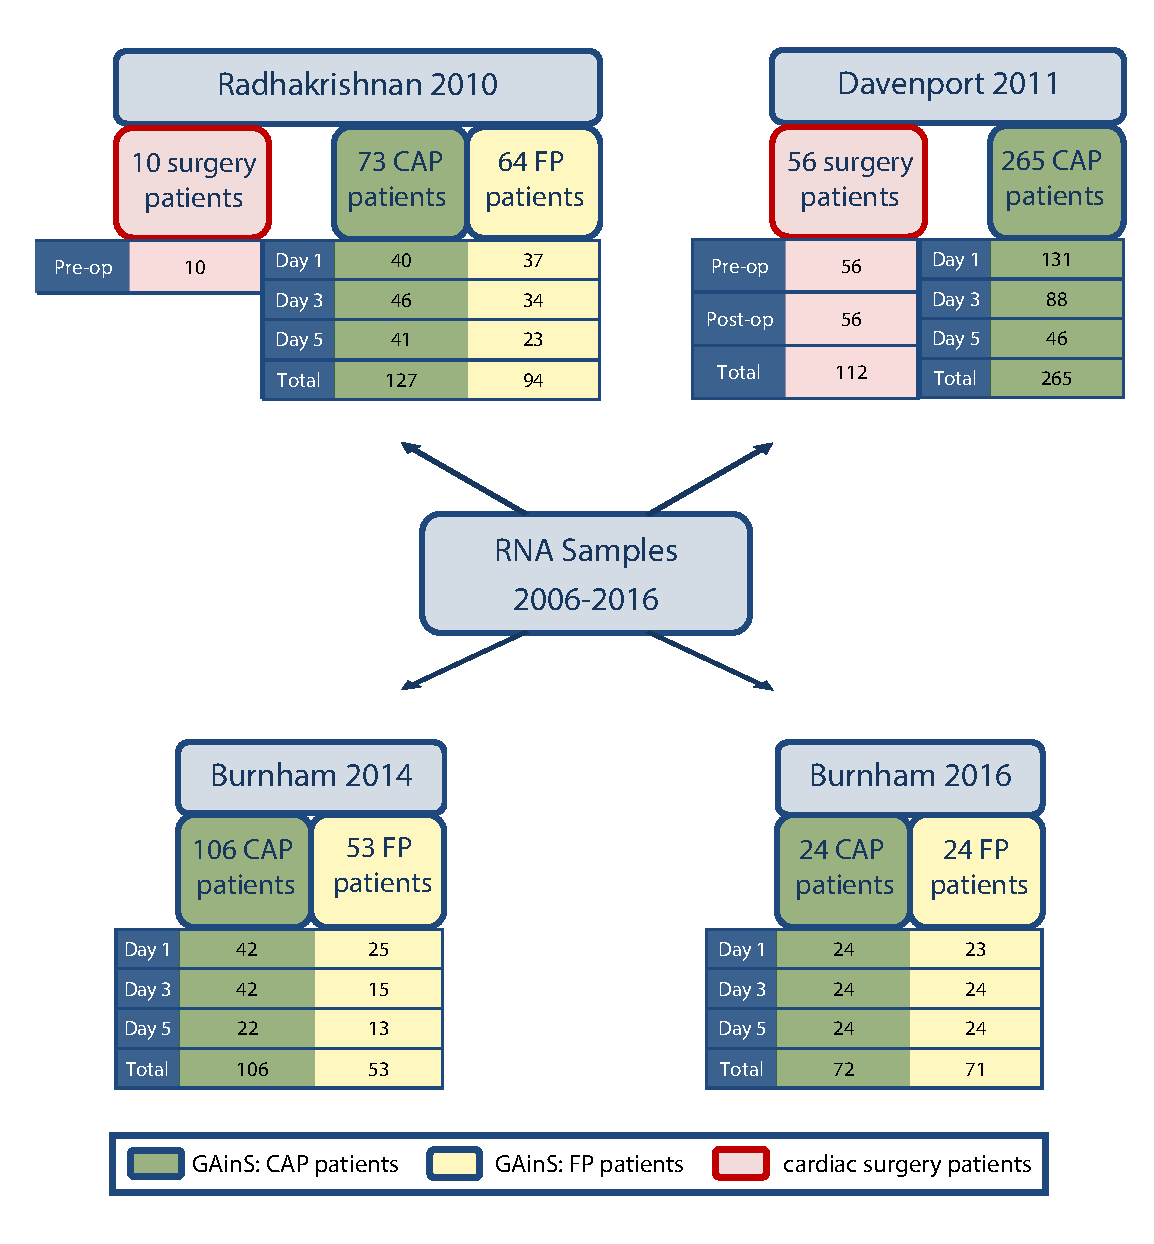
\includegraphics[width=\textwidth]{./Results1/CohortOverview}
\caption[Overview of GAinS gene expression cohorts]{\textbf{Overview of the GAinS gene expression datasets analysed in this thesis.} \\
The number of samples for which gene expression data are available following quality control is given for each of the four cohorts analysed in this thesis. This is subdivided according to the cause of sepsis (CAP (\emph{green}) or FP (\emph{yellow})), given the focus on source of infection in this chapter. Cohorts are named according to the person who generated the data and the year this was done. Samples from elective cardiac surgery patients (\emph{red}), taken before and after their operation by Eduardo Svoren, are also included in the Radhakrishnan 2010 and Davenport 2011 cohorts.}
\label{fig:CohortOverview}
\end{figure}

In this chapter, I analyse sepsis microarray gene expression data processed in several different batches over a six year period (Fig. \ref{fig:CohortOverview}). 

\section{Discussion}

\section{Conclusions}

The analysis presented in this chapter combines multiple transcriptomic datasets to compare the systemic inflammatory response across different sources. This demonstrates that a significant proportion of the sepsis transcriptomic response is shared between CAP and FP patients, although there is some specificity according to infection site. These findings may have implications for the management of sepsis, suggesting patient stratification and targeting treatment on the basis of cause of sepsis could be beneficial. In addition, future research and drug development may benefit from the use of more homogeneous cohorts. However, aspects of the transcriptomic response are shared across sepsis due to CAP and FP and sterile SIRS, indicating that findings in one SIRS subtype might be relevant to another and that similar treatment strategies could be considered. 
\chapter{General Discussion}
\label{ch:Discussion}
\textit{This chapter outlines the broader conclusions and future directions suggested by the work described in this thesis}

\startcontents[chapters]{\vspace{-1.4cm}}
\singlespacing
\printcontents[chapters]{}{1}{\section*{ }\setcounter{tocdepth}{1}}
\doublespacing
\vspace{0.5cm}

General intro

\section{A section}

\section{Limitations and future work}

\section{Conclusion}

Conclusions.
\appendix
\addcontentsline{toc}{chapter}{Appendices}

\singlespacing

\chapter{Materials and Methods}\label{app:Methods}
\begin{center}
\begin{landscape}

\begin{table}[htbp]
\begin{tabular}{|l|l|l|l|}
\hline
Organism               & Amplicon & Primer/probe                                                                           & Nucleotide sequence                                                                                                                                                               \\ \hline
\textit{S. pneumoniae} & 67 bp         & \begin{tabular}[c]{@{}l@{}}Taqman probe\\ Forward primer\\ Reverse primer\end{tabular} & \begin{tabular}[c]{@{}l@{}}5'-/5HEX/AAT GTT ACG/ZEN/CAA CTG ACG AG/3IABkFQ/-3'\\ 5'-GCT GTT TTA GCA GAT AGT GAG ATC GA-3'\\ 5'-TCC CAG TCG GTG CTG TCA-3'\end{tabular}            \\ \hline
Influenza A            & 185 bp        & \begin{tabular}[c]{@{}l@{}}Taqman probe\\ Forward primer\\ Reverse primer\end{tabular} & \begin{tabular}[c]{@{}l@{}}5'-/56-FAM/TGC AGT CCT/ZEN/CGC TCA CTG GGC ACG /3IABkFQ/-3'\\ 5'-AGG GCA TTY TGG ACA AAK CGT CTA-3'\\ 5'-GAC CRA TCC TGT CAC CTC TGA C-3'\end{tabular} \\ \hline
Epstein-Barr virus     & 75 bp         & \begin{tabular}[c]{@{}l@{}}Taqman probe\\ Forward primer\\ Reverse primer\end{tabular} & \begin{tabular}[c]{@{}l@{}}5'-/56-FAM/AGG GAG ACA/ZEN/CAT CTG GAC CAG AAG GC/3IABkFQ/-3'\\ 5'-TCT TTG AGG TCC ACT GCC G-3'\\ 5'-TAC AGG ACC TGG AAA TGG CC-3'\end{tabular}       \\ \hline
Cytomegalovirus        & 66 bp         & \begin{tabular}[c]{@{}l@{}}Taqman probe\\ Forward primer\\ Reverse primer\end{tabular} & \begin{tabular}[c]{@{}l@{}}5'-/56-FAM/TG GGC AAC C/ZEN/A CCG CAC TGA GG/3IABkFQ/-3'\\ 5'-TGG GCG AGG ACA ACG AA-3'\\ 5'-TGA GGC TGG GAA GCT GAC AT-3'\end{tabular}                \\ \hline
\end{tabular}
\medskip
\caption[Primer/probe sets used for the digital droplet PCR experiments]{\textbf{Primer/probe sets used for the digital droplet PCR experiments}}
\label{tab:ddPCRprobes}
\end{table}
\end{landscape}
\bigskip
\newpage





\chapter{Application of Metagenomic Sequencing to Sepsis Samples}
\label{app:Results1}


\begin{table}[]
\scalebox{0.7}{
\begin{tabular}{|l|l|}
\hline
\textbf{Virus family} & \textbf{Virus species}                                                                                                                                                                                                                                                                                   \\ \hline
Adenoviridae          & Human adenovirus                                                                                                                                                                                                                                                                                         \\ \hline
Arenaviridae          & \begin{tabular}[c]{@{}l@{}}Lassa virus\\ Lymphocytic choriomeningitis virus\end{tabular}                                                                                                                                                                                                                 \\ \hline
Coronaviridae         & \begin{tabular}[c]{@{}l@{}}Human coronavirus HKU1, NL63, OC43, 229E\\ Middle East respiratory syndrome coronavirus\\ Severe acute respiratory syndrome coronavirus\end{tabular}                                                                                                                          \\ \hline
Flaviviridae          & \begin{tabular}[c]{@{}l@{}}Dengue virus\\ Japanese encephalitis virus\\ Murray Valley encephalitis virus\\ St Louis encephalitis virus\\ Tick-borne encephalitis virus\\ West Nile virus\\ Yellow fever virus\\ Zika virus\end{tabular}                                                                  \\ \hline
Herpesviridae         & \begin{tabular}[c]{@{}l@{}}Human herpesvirus 3 (Varicella zoster virus)\\ Human herpesvirus 4 (Epstein Barrvirus)\\ Human herpesvirus 5 (Cytomegalovirus)\\ Human herpesvirus 6-7 (Roseolovirus)\\ Human herpesvirus 8 (Kaposi's sarcoma-associated herpesvirus)\\ Herpes simplex virus 1-2\end{tabular} \\ \hline
Orthomyxoviridae      & Influenza virus A-C                                                                                                                                                                                                                                                                                      \\ \hline
Paramyxoviridae       & \begin{tabular}[c]{@{}l@{}}Hendra henipavirus\\ Human metapneumovirus \\ Humanparainfluenzavirus1-5\\ Measles morbilivirus\\ Mumps rubulavirus\\ Nipah henipavirus\\ Respiratory syncytial virus \\ Sosugavirus\end{tabular}                                                                             \\ \hline
Parvoviridae          & \begin{tabular}[c]{@{}l@{}}Human bocavirus\\ Human parvovirus B19\\ Human parvovirus 4\\ Primate erythroparvovirus 1\\ Primate tetraparvovirus 1\end{tabular}                                                                                                                                            \\ \hline
Peribunyaviridae      & California encephalitis virus                                                                                                                                                                                                                                                                            \\ \hline
Phenuiviridae         & \begin{tabular}[c]{@{}l@{}}Rift valley fever virus\\ Sandfly fever Naples virus\\ Sandfly fever Sicilian virus\end{tabular}                                                                                                                                                                              \\ \hline
Picornaviridae        & \begin{tabular}[c]{@{}l@{}}Cardiovirus A-B\\ Coxsackie A virus\\ ECHO virus\\ Enterovirus A, B, D\\ Hepatitis A virus\\ Parechovirus A-B \\ Rhinovirus A-C\\ Rosavirus A\\ Salivivirus\end{tabular}                                                                                                      \\ \hline
Polyomaviridae        & \begin{tabular}[c]{@{}l@{}}BK virus\\ JC polyomavirus\end{tabular}                                                                                                                                                                                                                                       \\ \hline
Reoviridae            & Rotavirus A-C                                                                                                                                                                                                                                                                                            \\ \hline
Rhabdovirus           & \begin{tabular}[c]{@{}l@{}}Australian bat lyssavirus\\ Duvenhage lyssavirus\\ European bat lyssavirus 1-2\\ Lagos bat lyssavirus\\ Mokola lyssavirus\\ Rabies lyssavirus\end{tabular}                                                                                                                    \\ \hline
Togaviridae           & \begin{tabular}[c]{@{}l@{}}Chikungunya virus\\ Eastern equine encephalitis virus\\ Rubella virus\\ Venezuelan equine encephalitis virus\\ Western equine encephalitis virus\end{tabular}                                                                                                                 \\ \hline
\end{tabular}
}
\caption[Enrichment Probe Set Viruses]{\textbf{Viruses included in enrichment probe set}}
\label{tab:ProbeSetViruses}
\end{table}

\begin{table}[]
\begin{tabular}{|l|l|}
\hline
\textbf{Bacterial genus}  & \textbf{Bacterial species}                                                             \\ \hline
\textit{Acinetobacter}    & \textit{\begin{tabular}[c]{@{}l@{}}baumanii\\ calcoaceticus\end{tabular}}              \\ \hline
\textit{Bartonella}       & \textit{henselae}                                                                      \\ \hline
\textit{Bordetella}       & \textit{pertussis}                                                                     \\ \hline
\textit{Borrelia}         & \textit{burgdorferi}                                                                   \\ \hline
\textit{Brucella}         & \textit{}                                                                              \\ \hline
\textit{Burkholderia}     & \textit{cepacia}                                                                       \\ \hline
\textit{Chlamydophila}    & \textit{\begin{tabular}[c]{@{}l@{}}pneumoniae\\ psittaci\end{tabular}}                 \\ \hline
\textit{Coxiella}         & \textit{burnetii}                                                                      \\ \hline
\textit{Enterobacter}     & \textit{\begin{tabular}[c]{@{}l@{}}aerogenes\\ cloacae\end{tabular}}                   \\ \hline
\textit{Escherichia}      & \textit{coli}                                                                          \\ \hline
\textit{Haemophilus}      & \textit{\begin{tabular}[c]{@{}l@{}}influenzae\\ parainfluenzae\end{tabular}}           \\ \hline
\textit{Klebsiella}       & \textit{\begin{tabular}[c]{@{}l@{}}pneumoniae\\ oxytoca\end{tabular}}                  \\ \hline
\textit{Legionella}       & \textit{pneumophila}                                                                   \\ \hline
\textit{Leptospira}       & \textit{}                                                                              \\ \hline
\textit{Listeria}         & \textit{monocytogenes}                                                                 \\ \hline
\textit{Moraxella}        & \textit{catarrhalis}                                                                   \\ \hline
\textit{Mycobacterium}    & \textit{\begin{tabular}[c]{@{}l@{}}avium\\ intracellulare\\ tuberculosis\end{tabular}} \\ \hline
\textit{Mycoplasma}       & \textit{pneumoniae}                                                                    \\ \hline
\textit{Neisseria}        & \textit{meningitidis}                                                                  \\ \hline
\textit{Nocardia}         & \textit{}                                                                              \\ \hline
\textit{Pseudomonas}      & \textit{aeruginosa}                                                                    \\ \hline
\textit{Serratia}         & \textit{marcescens}                                                                    \\ \hline
\textit{Staphylococcus}   & \textit{aureus}                                                                        \\ \hline
\textit{Stenotrophomonas} & \textit{maltophilia}                                                                   \\ \hline
\textit{Streptococcus}    & \textit{\begin{tabular}[c]{@{}l@{}}agalactiae\\ pneumoniae\\ pyogenes\end{tabular}}    \\ \hline
\textit{Treponema}        & \textit{pallidum}                                                                      \\ \hline
\end{tabular}
\caption[Enrichment Probe Set Bacteria]{\textbf{Bacteria included in enrichment probe set}}
\label{tab:ProbeSetBacteria}
\end{table}




\begin{landscape}


\begin{table}[]
\centering
\caption[Viral Multiplex Reference]{Viral Multiplex Reference reagent 11/242 (UK NIBSC). This reference set included 25 viruses of various nucleic acid types, envelope types and genome sizes. 21/25 viruses had corresponding enrichment probes in our probe panel. (Adapted from Mee et al.)
\label{tab:VMR}\\
{\bf }}
\scalebox{0.85}{
\begin{tabular}{|l|l|l|l|l|l|l|}
\hline
Group                      & Family                            & Species/serotype               & Envelope             & Genome size & Included in probeset & Concentration (log10 copies/ml) \\ \hline
\multirow{7}{*}{dsDNA}     & \multirow{2}{*}{Adenoviridae}     & Adenovirus 2                   & \multirow{2}{*}{No}  & 35.9        & Yes                  & NA                                           \\ \cline{3-3} \cline{5-7} 
                           &                                   & Adenovirus 41                  &                      & 34.2        & Yes                  & NA                                           \\ \cline{2-7} 
                           & \multirow{5}{*}{Herpesviridae}    & Human herpesvirus 1            & \multirow{5}{*}{Yes} & 151.2       & Yes                  & NA                                           \\ \cline{3-3} \cline{5-7} 
                           &                                   & Human herpesvirus 2            &                      & 154.7       & Yes                  & NA                                           \\ \cline{3-3} \cline{5-7} 
                           &                                   & Human herpesvirus 3 (VZV)      &                      & 124.8       & Yes                  & NA                                           \\ \cline{3-3} \cline{5-7} 
                           &                                   & Human herpesvirus 4 (EBV)      &                      & 171.7       & Yes                  & 3.88                                         \\ \cline{3-3} \cline{5-7} 
                           &                                   & Human herpesvirus 5 (CMV)      &                      & 233.7       & Yes                  & 4.66                                         \\ \hline
dsRNA                      & Reoviridae                        & Rotavirus A                    & No                   & 18.5        & Yes                  & 6.76                                         \\ \hline
\multirow{8}{*}{ssRNA (+)} & Astroviridae                      & Astrovirus                     & No                   & 6.8         & No                   & NA                                           \\ \cline{2-7} 
                           & \multirow{3}{*}{Caliciviridae}    & Norovirus GI                   & \multirow{3}{*}{No}  & 7.6         & No                   & NA                                           \\ \cline{3-3} \cline{5-7} 
                           &                                   & Norovirus GII                  &                      & 7.5         & No                   & NA                                           \\ \cline{3-3} \cline{5-7} 
                           &                                   & Sapovirus C12                  &                      & 7.5         & No                   & NA                                           \\ \cline{2-7} 
                           & Coronaviridae                     & Coronavirus 229E               & Yes                  & 27.2        & Yes                  & NA                                           \\ \cline{2-7} 
                           & \multirow{3}{*}{Picornaviridae}   & Coxsackievirus B4              & \multirow{3}{*}{No}  & 7.4         & Yes                  & NA                                           \\ \cline{3-3} \cline{5-7} 
                           &                                   & Rhinovirus A39                 &                      & 7.1         & Yes                  & NA                                           \\ \cline{3-3} \cline{5-7} 
                           &                                   & Parechovirus 3                 &                      & 7.2         & Yes                  & 7.07                                         \\ \hline
\multirow{9}{*}{ssRNA (-)} & \multirow{3}{*}{Orthomyxoviridae} & Influenza A virus H1N1         & \multirow{3}{*}{Yes} & 13.2        & Yes                  & NA                                           \\ \cline{3-3} \cline{5-7} 
                           &                                   & Influenza A virus H3N2         &                      & 13.6        & Yes                  & NA                                           \\ \cline{3-3} \cline{5-7} 
                           &                                   & Influenza B virus              &                      & 14.2        & Yes                  & NA                                           \\ \cline{2-7} 
                           & \multirow{6}{*}{Paramyxoviridae}  & Metapneumovirus A              & \multirow{6}{*}{Yes} & 13.3        & Yes                  & NA                                           \\ \cline{3-3} \cline{5-7} 
                           &                                   & Parainfluenzavirus 1           &                      & 15.5        & Yes                  & NA                                           \\ \cline{3-3} \cline{5-7} 
                           &                                   & Parainfluenzavirus 2           &                      & 15.7        & Yes                  & NA                                           \\ \cline{3-3} \cline{5-7} 
                           &                                   & Parainfluenzavirus 3           &                      & 15.4        & Yes                  & NA                                           \\ \cline{3-3} \cline{5-7} 
                           &                                   & Parainfluenzavirus 4           &                      & 17.4        & Yes                  & NA                                           \\ \cline{3-3} \cline{5-7} 
                           &                                   & Respiratory syncytial virus A2 &                      & 15.2        & Yes                  & 3.75                                         \\ \hline
\small
\end{tabular}
}
\end{table}


\end{landscape}

\clearpage

\end{center}

\chapter{Improved Classification of Microbiological Aetiology in Sepsis}
\label{ch:AppResults2}
\begin{figure}[htbp]
\centering
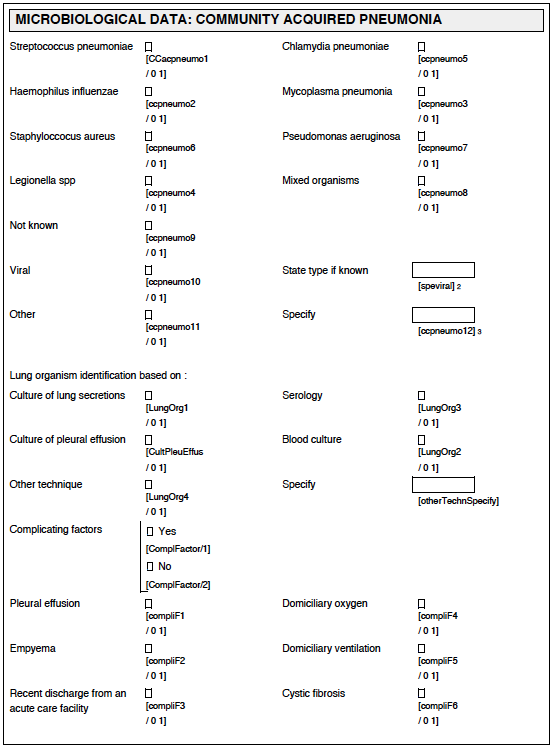
\includegraphics[scale=0.7]{./Appendices/Images/eCRF1.png}
\end{figure}

\begin{figure}[htbp]
\centering
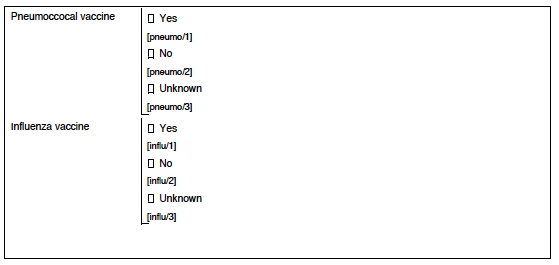
\includegraphics[scale=0.7]{./Appendices/Images/eCRF2.png}
\caption[Electronic case record form]{\textbf{GAinS electronic case record form: microbiology section}}
\label{fig:eCRF}
\end{figure}

\chapter{Integration of Microbiology with the Host Response}\label{ch:AppResults3}

\begin{table}[]
\begin{center}
\begin{tabular}{lll}
\textbf{Gene}      & \textbf{log2(fold change)} & \textbf{FDR} \\
\textit{IGLL1}     & 0.79                       & 4.02E-03     \\
\textit{CDC20}     & 0.62                       & 4.51E-03     \\
\textit{CACNA2D3}  & -0.63                      & 5.21E-03     \\
\textit{TXNDC5}    & 0.75                       & 8.48E-03     \\
\textit{IGKV3D-20} & 0.78                       & 9.23E-03     \\
\textit{KIAA0101}  & 0.59                       & 1.28E-02     \\
\textit{IGKV1D-33} & 0.61                       & 1.33E-02     \\
\textit{IGJ}       & 0.83                       & 1.33E-02     \\
\textit{PRTN3}     & 0.66                       & 4.68E-02    
\end{tabular}
\end{center}
\caption[Differentially expressed genes in EBV reactivation]{\textbf{Summary of differentially expressed genes in EBV-positive vs EBV-negative individuals.} Nine genes were significant at fold-change $>$1.5 and FDR $<$0.05.} 
\label{tab:ebv-de-genes}
\end{table}

\begin{table}[]
\begin{center}
\begin{tabular}{lll}
\textbf{Gene}      & \textbf{log2(fold change)} & \textbf{FDR} \\
\textit{IGLL1}     & 0.85                       & 1.15E-03     \\
\textit{TXNDC5}    & 0.81                       & 2.43E-03     \\
\textit{IGKV3D-20} & 0.84                       & 2.54E-03     \\
\textit{IGKV1D-33} & 0.66                       & 3.38E-03     \\
\textit{CDC20}     & 0.59                       & 3.98E-03     \\
\textit{IGJ}       & 0.89                       & 4.06E-03     \\
\textit{MGC29506}  & 0.61                       & 5.96E-03     \\
\textit{TNFRSF17}  & 0.63                       & 1.32E-02     \\
\textit{DEFA1B} & 0.82                       & 3.11E-02     \\
\textit{PRTN3}     & 0.66                       & 3.87E-02     \\
\textit{DEFA4}     & 0.75                       & 4.19E-02     \\
\textit{CEACAM6}   & 0.63                       & 4.82E-02    
\end{tabular}
\end{center}
\caption[Differentially expressed genes in EBV reactivation with SRS as a covariate]{\textbf{Summary of differentially expressed genes in EBV-positive vs EBV-negative individuals with SRS included as a covariate in the linear model.} Twelve genes were significant at fold-change $>$1.5 and FDR $<$0.05.} 
\label{tab:ebv-de-genes-srs}
\end{table}



\begin{table}
\begin{center}
\scalebox{0.9}{
\begin{tabular}{lll}
\textbf{Gene}      & \textbf{log2(fold change)} & \textbf{FDR} \\
\textit{IFI27}     & 3.10           & 6.88E-07           \\
\textit{IMPA2}     & -0.64          & 1.86E-04           \\
\textit{C3ORF54}   & 0.74           & 6.59E-04           \\
\textit{SPATS2L}   & 1.02           & 6.59E-04           \\
\textit{LOC554203} & 0.59           & 6.91E-04           \\
\textit{HERC6}     & 0.94           & 8.17E-04           \\
\textit{JUP}       & 1.28           & 9.63E-04           \\
\textit{TIMM10}    & 1.33           & 1.03E-03           \\
\textit{SRC}       & 0.77           & 1.03E-03           \\
\textit{HES4}      & 1.04           & 1.03E-03           \\
\textit{LGALS3BP}  & 0.82           & 1.03E-03           \\
\textit{RASGRP3}   & 0.75           & 1.03E-03           \\
\textit{TGIF2}     & 0.64           & 1.03E-03           \\
\textit{MT1A}      & 0.89           & 1.03E-03           \\
\textit{C9ORF91}   & 0.75           & 1.03E-03           \\
\textit{OAS1}      & 1.42           & 1.08E-03           \\
\textit{SCO2}      & 0.92           & 1.08E-03           \\
\textit{HS.125087} & 1.21           & 1.08E-03           \\
\textit{PARP12}    & 1.07           & 1.08E-03           \\
\textit{EPSTI1}    & 2.02           & 1.08E-03           \\
\textit{OAS2}      & 1.57           & 1.08E-03           \\
\textit{IFI44L}    & 2.42           & 1.08E-03           \\
\textit{SP140}     & 0.78           & 1.08E-03           \\
\textit{LY6E}      & 1.69           & 1.11E-03           \\
\textit{CXCL10}    & 0.78           & 1.16E-03           \\
\textit{TMCO3}     & -0.70          & 1.21E-03           \\
\textit{HS.72010}  & 0.63           & 1.28E-03           \\
\textit{XAF1}      & 1.44           & 1.28E-03           \\
\textit{IFI44}     & 1.68           & 1.33E-03           \\
\textit{RNASE1}    & 0.94           & 1.36E-03           \\
\textit{GALM}      & 0.85           & 1.45E-03           \\
\textit{IFIT3}     & 1.57           & 1.45E-03           \\
\textit{RSAD2}     & 1.81           & 1.84E-03           \\
\textit{LAMP3}     & 0.72           & 1.99E-03           \\
\textit{HS.386275} & 0.70           & 1.99E-03           \\
\textit{PLB1}      & -0.74          & 2.02E-03           \\
\textit{MT2A}      & 1.00           & 2.14E-03           \\
\textit{SERPING1}  & 1.50           & 2.14E-03           \\
\textit{OAS3}      & 1.66           & 2.14E-03           \\
\textit{CDKN1A}    & 0.71           & 2.14E-03           \\
\textit{LHFPL2}    & 0.68           & 2.30E-03           \\
\textit{BTN3A3}    & 0.85           & 2.47E-03           \\
\textit{PARP14}    & 0.95           & 2.52E-03           \\
\textit{IFIT5}     & 0.97           & 2.57E-03           \\
\textit{FHL2}      & 0.61           & 2.60E-03           \\
\textit{CXCL16}    & -0.63          & 2.93E-03           \\
\textit{SIGLEC10}  & -0.88          & 3.13E-03           \\
\textit{NLRC4}     & -0.67          & 3.55E-03           \\
\textit{ISG15}     & 1.68           & 3.59E-03           \\
\textit{ZNF684}    & 0.60           & 3.63E-03                  


\end{tabular}}
\end{center}
\caption[Differentially expressed genes in viral infection]{\textbf{Summary of differentially expressed genes in viral vs bacterial infection.} The top 50 most significantly differentially expressed genes are listed here.} 
\label{tab:vb-de-genes}
\end{table}

\begin{table}[]
\begin{center}
\scalebox{0.9}{
\begin{tabular}{lll}
\textbf{Gene}      & \textbf{log2(fold change)} & \textbf{FDR} \\
\textit{IFI27}     & 3.52                       & 1.3E-06      \\
\textit{JUP}       & 1.68                       & 2.0E-04      \\
\textit{C3ORF54}   & 0.90                       & 4.7E-04      \\
\textit{NPL}       & -0.66                      & 7.9E-04      \\
\textit{SPATS2L}   & 1.17                       & 1.1E-03      \\
\textit{CBL}       & -0.68                      & 1.4E-03      \\
\textit{IMPA2}     & -0.67                      & 1.7E-03      \\
\textit{HERC6}     & 1.01                       & 4.8E-03      \\
\textit{LGALS3BP}  & 0.89                       & 5.1E-03      \\
\textit{HES4}      & 1.12                       & 6.0E-03      \\
\textit{MT1A}      & 0.98                       & 6.2E-03      \\
\textit{BCAT1}     & -1.20                      & 7.0E-03      \\
\textit{RASGRP3}   & 0.80                       & 7.0E-03      \\
\textit{ECHDC3}    & -1.25                      & 7.2E-03      \\
\textit{CDC123}    & -0.62                      & 7.2E-03      \\
\textit{MTE}       & 0.64                       & 7.2E-03      \\
\textit{SCO2}      & 1.00                       & 7.2E-03      \\
\textit{SP140}     & 0.83                       & 7.2E-03      \\
\textit{LOC389386} & 0.66                       & 7.2E-03      \\
\textit{GALM}      & 0.95                       & 7.2E-03      \\
\textit{UBQLNL}    & 0.60                       & 7.2E-03      \\
\textit{SOCS2}     & 0.82                       & 7.2E-03      \\
\textit{LY6E}      & 1.83                       & 7.2E-03      \\
\textit{HS.125087} & 1.25                       & 7.2E-03      \\
\textit{OAS2}      & 1.69                       & 7.2E-03      \\
\textit{NUDT5}     & -0.65                      & 7.5E-03      \\
\textit{MT2A}      & 1.12                       & 8.0E-03      \\
\textit{IFI44L}    & 2.55                       & 8.0E-03      \\
\textit{OAS1}      & 1.48                       & 8.0E-03      \\
\textit{ADARB1}    & 0.70                       & 8.0E-03      \\
\textit{LAMP3}     & 0.79                       & 8.0E-03      \\
\textit{LOC401845} & 0.62                       & 8.0E-03      \\
\textit{PARP12}    & 1.11                       & 8.0E-03      \\
\textit{CDKN1A}    & 0.80                       & 8.0E-03      \\
\textit{SLC31A2}   & -0.73                      & 8.0E-03      \\
\textit{CXCL10}    & 0.78                       & 8.0E-03      \\
\textit{FHL2}      & 0.70                       & 8.0E-03      \\
\textit{XAF1}      & 1.51                       & 8.0E-03      \\
\textit{HIST1H4E}  & 0.59                       & 8.0E-03      \\
\textit{DUSP5}     & 0.66                       & 8.1E-03      \\
\textit{TGIF2}     & 0.65                       & 8.6E-03      \\
\textit{PDE9A}     & 0.73                       & 8.9E-03      \\
\textit{HS.72010}  & 0.66                       & 8.9E-03      \\
\textit{IFI44}     & 1.77                       & 9.4E-03      \\
\textit{TIMM10}    & 1.28                       & 9.4E-03      \\
\textit{LOC652694} & 1.34                       & 9.8E-03      \\
\textit{RAB11FIP3} & 0.60                       & 9.8E-03      \\
\textit{CD69}      & 0.86                       & 1.0E-02      \\
\textit{SRC}       & 0.74                       & 1.0E-02      \\
\textit{OAS3}      & 1.79                       & 1.0E-02     
\end{tabular}}
\end{center}
\caption[Differentially expressed genes in influenza infection]{\textbf{Summary of differentially expressed genes in influenza vs bacterial infection.} The top 50 most significantly differentially expressed genes are listed here.}
\label{tab:flu-de-genes}
\end{table}

\newpage
\addcontentsline{toc}{chapter}{Bibliography}

\singlespacing
\setlength\bibitemsep{\itemsep}
\printbibliography

\end{document}